
    \begin{frame}{How good is the Taylor approximation?}

        \[
            f(\cdot, \bm \theta) \approx \hat{f}(\cdot, \bm \theta) = f(\cdot, \bm m) + \mathcal{J}(\cdot, \bm m)(\bm \theta - \bm m) 
        \]

        \textbf{Advantages}: 
        \begin{enumerate}
            \item The mean of the approximation is in the support of the function-space distribution.
            \item Does not rely on taking samples of the prior, avoiding an hyperparameter that depends on the dimensionality of the data.
        \end{enumerate}
        \textbf{Disadvantages:}
        \begin{enumerate}
            \item The approximation is degenerate when \(\mathbb{E}_{P}[\bm \theta] = \bm m = \bm 0\).
        \end{enumerate}
    \end{frame}
    \begin{frame}
        Assume that 
        \[
        f(\cdot, (\bm w_1, \bm w_2)) = \bm w_2 \tanh (\bm w_1 \mathbf x), \quad \text{and} \quad 
        \mathbb{E}_{P}[(\bm w_1, \bm w_2)] =(\bm m_1, \bm m_2) = (\bm 0, \bm 0)\,.
        \]
        then
        \[
            \mathcal{J}(\mathbf x, \bm m) = \frac{\partial f(\mathbf x,(\bm w_1, \bm w_2))}{\partial (\bm w_1, \bm w_2)}(\bm m_1, \bm m_2) = 
            \begin{pmatrix}
                \bm m_2 (1 - \tanh(\bm m_1 \mathbf x)^2)\mathbf x\\
                \tanh (\bm m_1 \mathbf x)
            \end{pmatrix}
             =  \begin{pmatrix}
                \bm 0 \\
                \bm 0
            \end{pmatrix}
        \]
        Meaning that
        \[
            f(\cdot, \bm \theta) \approx \hat{f}(\cdot, \bm \theta) = f(\cdot, \bm m) + \cancel{\mathcal{J}(\cdot, \bm m)(\bm \theta - \bm m)}\,.
        \]

        \textbf{However}, this can be solved using random initialization of the mean values of the prior distribution \(P_{\bm \Theta}\).
    \end{frame}
    
    \begin{frame}{Is the Taylor GP close to the true GP?}

        We want to test if in cases where \(P(f(\cdot))\) is a GP, the Taylor approximation GP is a good approximation. 

        \textbf{Approach}. Create a Bayesian Neural Network whose implicit distribution equals that of a Gaussian Process.

        \begin{enumerate}
            \item \textbf{Squared exponential Kernel}: Single hidden layer BNN with cos activation and infinite width. Gaussian weights and uniform biases.
            \item \textbf{Gaussian c.d.f activation}: Single hidden layer BNN with Gaussian c.d.f activation.
        \end{enumerate}
    \end{frame}

    \begin{frame}{GP approximation}
        Let 
        \[
            f(\mathbf x) = \frac{1}{\sqrt{H}}\bm w_2^T \phi(\bm w_1^T \mathbf x + \bm b_1) + b_2\,,
        \]
        where the dimensionality of the parameter verctors is \(H\)
        \[
            \begin{aligned}
            \bm w_1 &\sim \mathcal{N}(\bm m_{w_1}, \bm \sigma_{w_1} \bm I),\quad &\bm b_1 \sim \mathcal{N}(\bm m_{b_1}, \bm \sigma_{b_1} \bm I)\,,\\
            \bm w_2 &\sim \mathcal{N}(\bm m_{w_2}, \bm \sigma_{w_2} \bm I),\quad &\bm b_2 \sim \mathcal{N}(\bm m_{b_2}, \bm \sigma_{b_2} \bm I)\,.\\
            \end{aligned}
        \]
        The distribution of \(f(\mathbf x)\) tends to a GP when \(H \to \infty\). The mean and covariance of \(f(\mathbf x)\) can be computed using 1-dimensional quadrature.

        In practise, \(H = 20\) is enough to approximate the GP. 
    \end{frame}

    \begin{frame}{Showing that \(H = 20\) is good enough}
        \begin{center}
            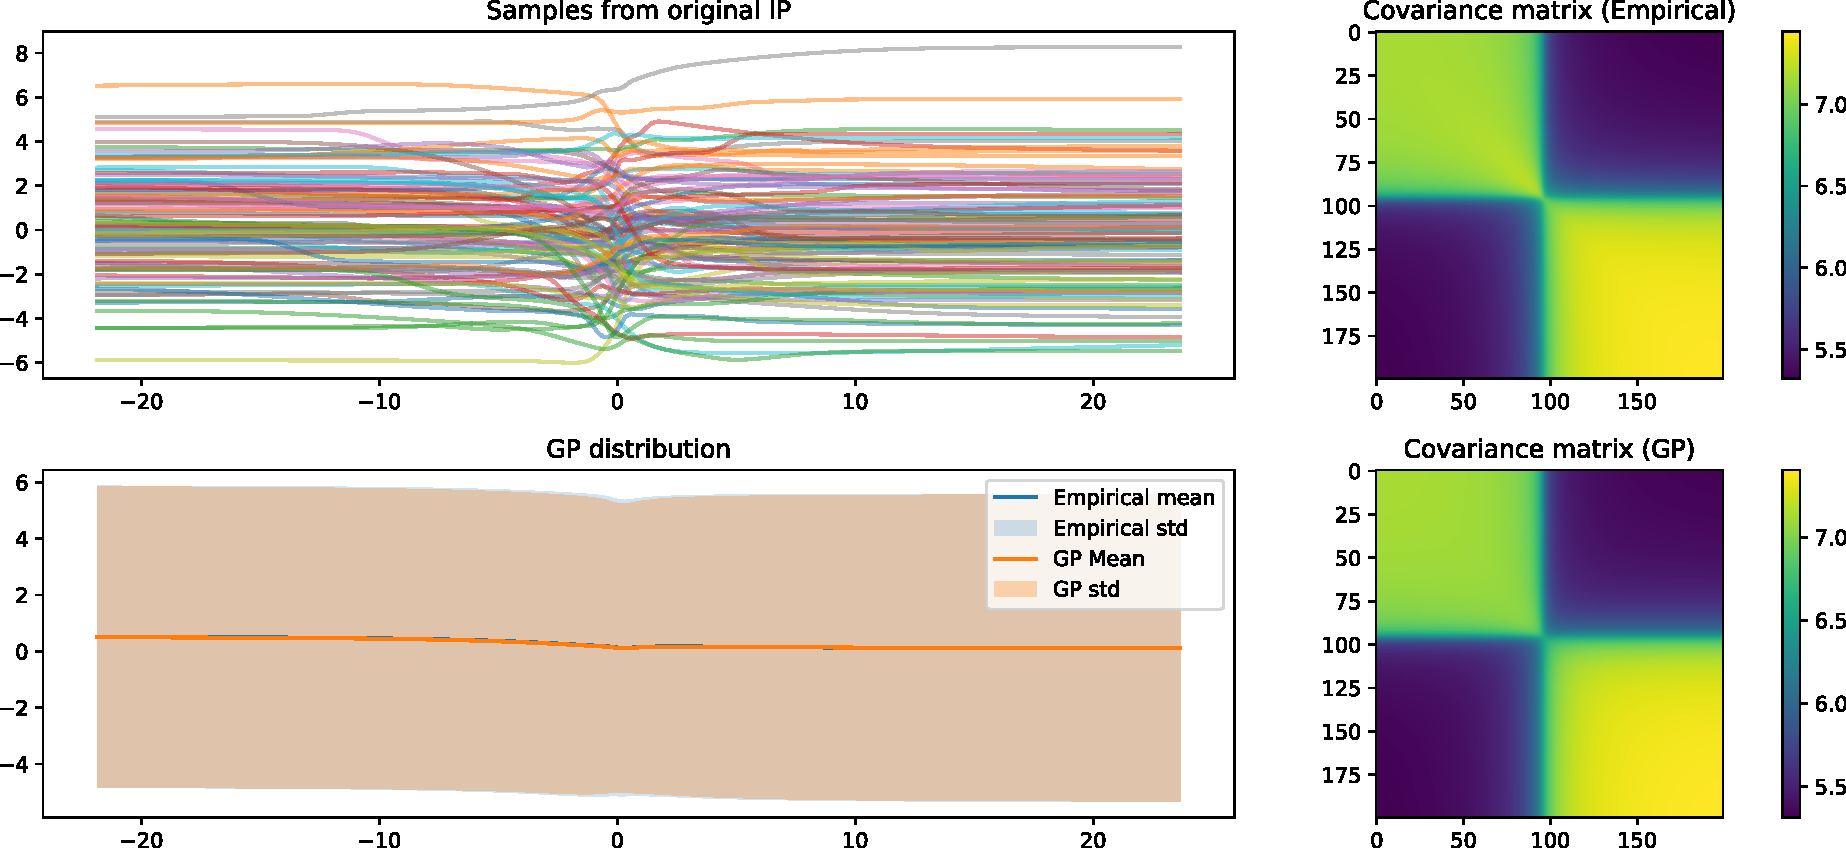
\includegraphics[width=0.95\textwidth]{imgs/GP_cov.pdf}
        \end{center}
    \end{frame}

    \begin{frame}
        \begin{center}
            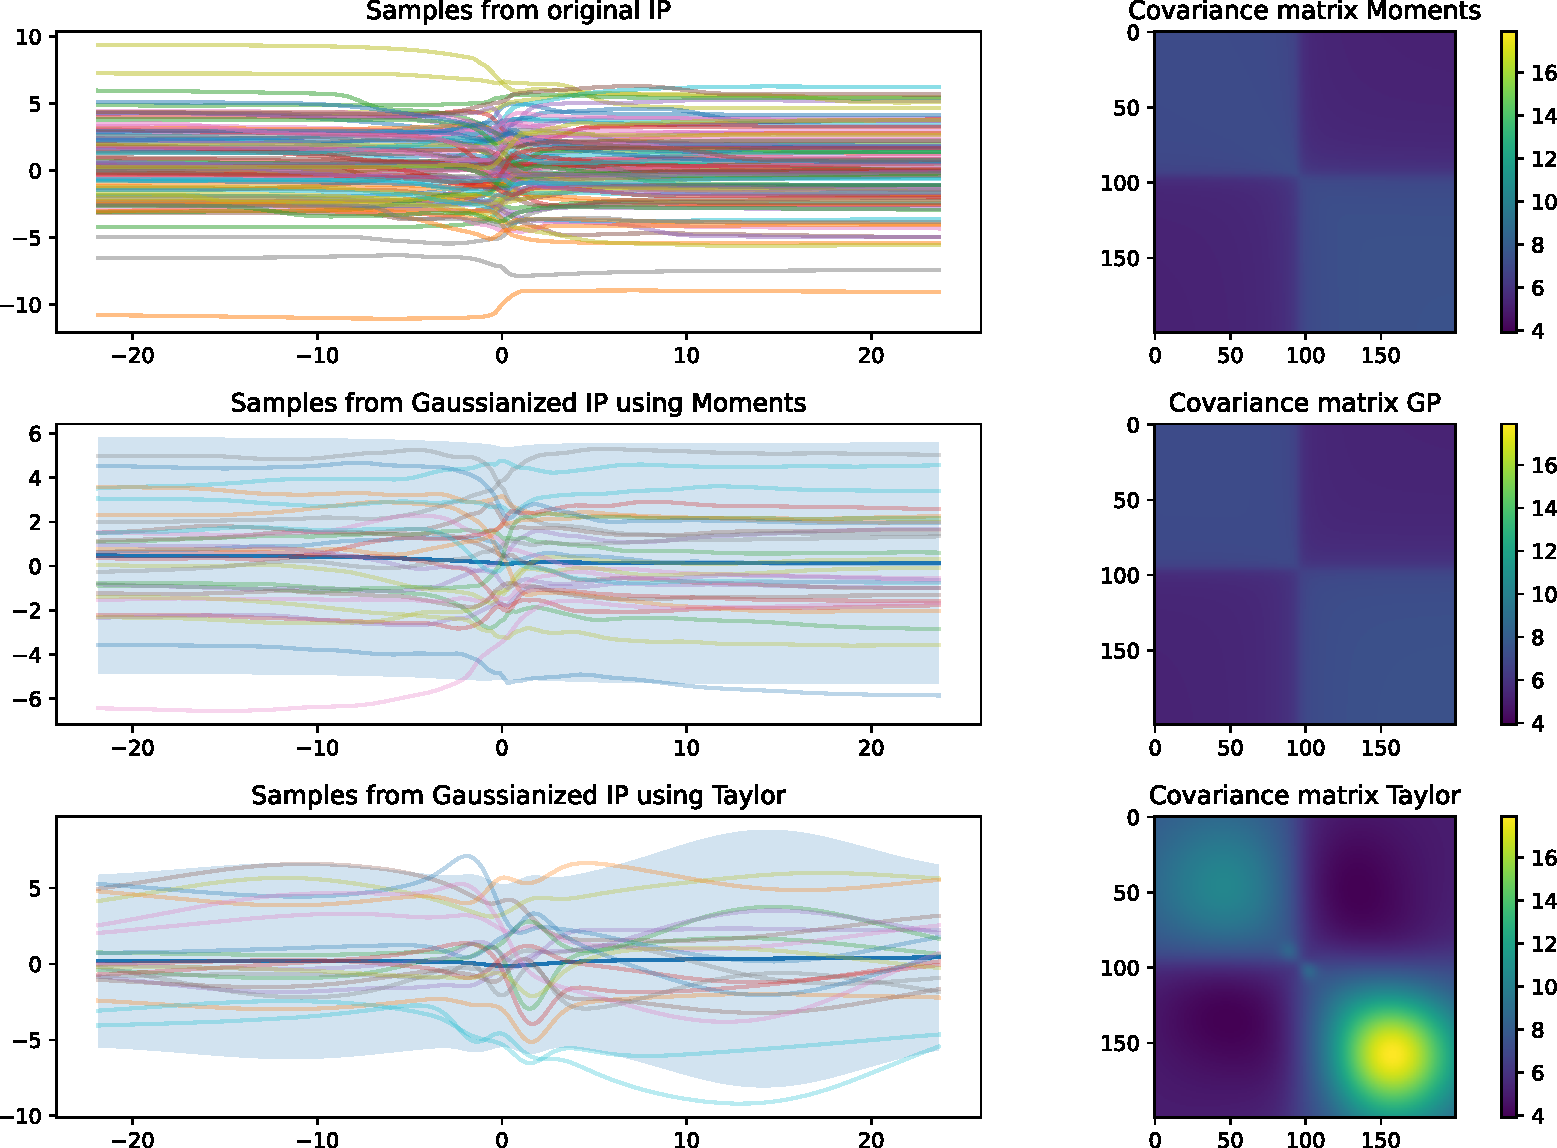
\includegraphics[width=0.8\textwidth]{imgs/GP_taylor.pdf}
        \end{center}
    \end{frame}

    \begin{frame}{Exact posterior distributions}
        We are considering three main models based on the stochastic function 
        \[
            f(\mathbf x) = \frac{1}{\sqrt{H}}\bm w_2^T \phi(\bm w_1^T \mathbf x + \bm b_1) + b_2\,.
        \]
        \begin{enumerate}
            \item The \textbf{exact GP} of the stochastic function.
            \item A GP where the mean and covariance are estimated using \textbf{samples} from the stochastic function.
            \item A GP where the mean and covariance are the ones obtained from the \textbf{Taylor} approximation.
        \end{enumerate}

        We are testing these three methods on a toy 1-D dataset where the exact GP posteriors can be computed.
    \end{frame}

    \begin{frame}
        \begin{center}
        \begin{tabular}{ c c }
         Theoretical GP & GP Samples \\ 
         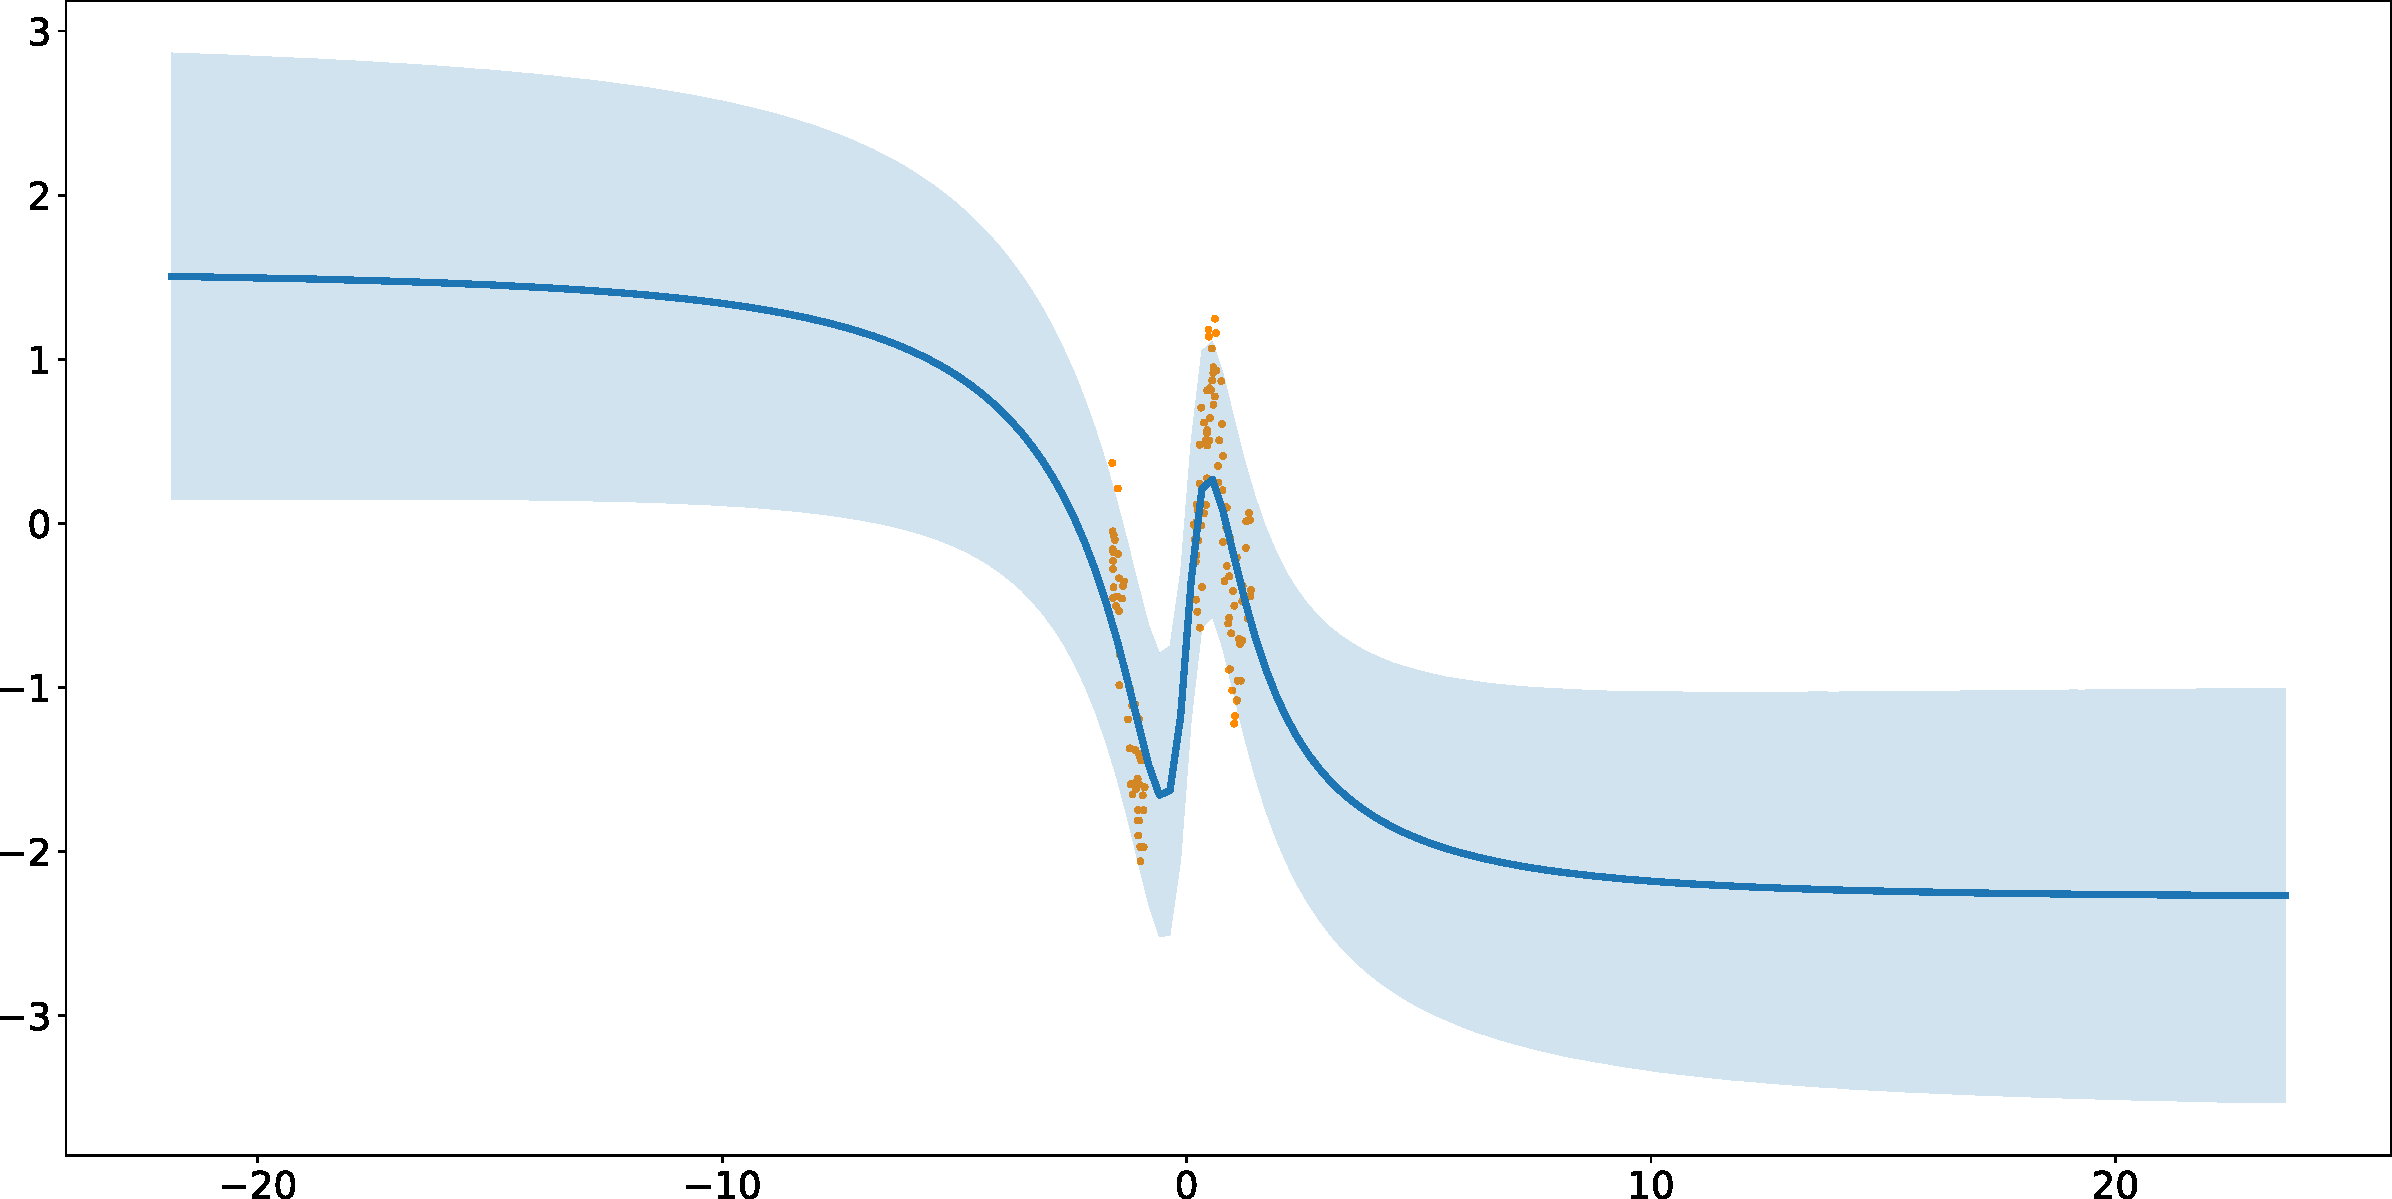
\includegraphics[width=0.49\textwidth]{imgs/Exact_GP.pdf} & 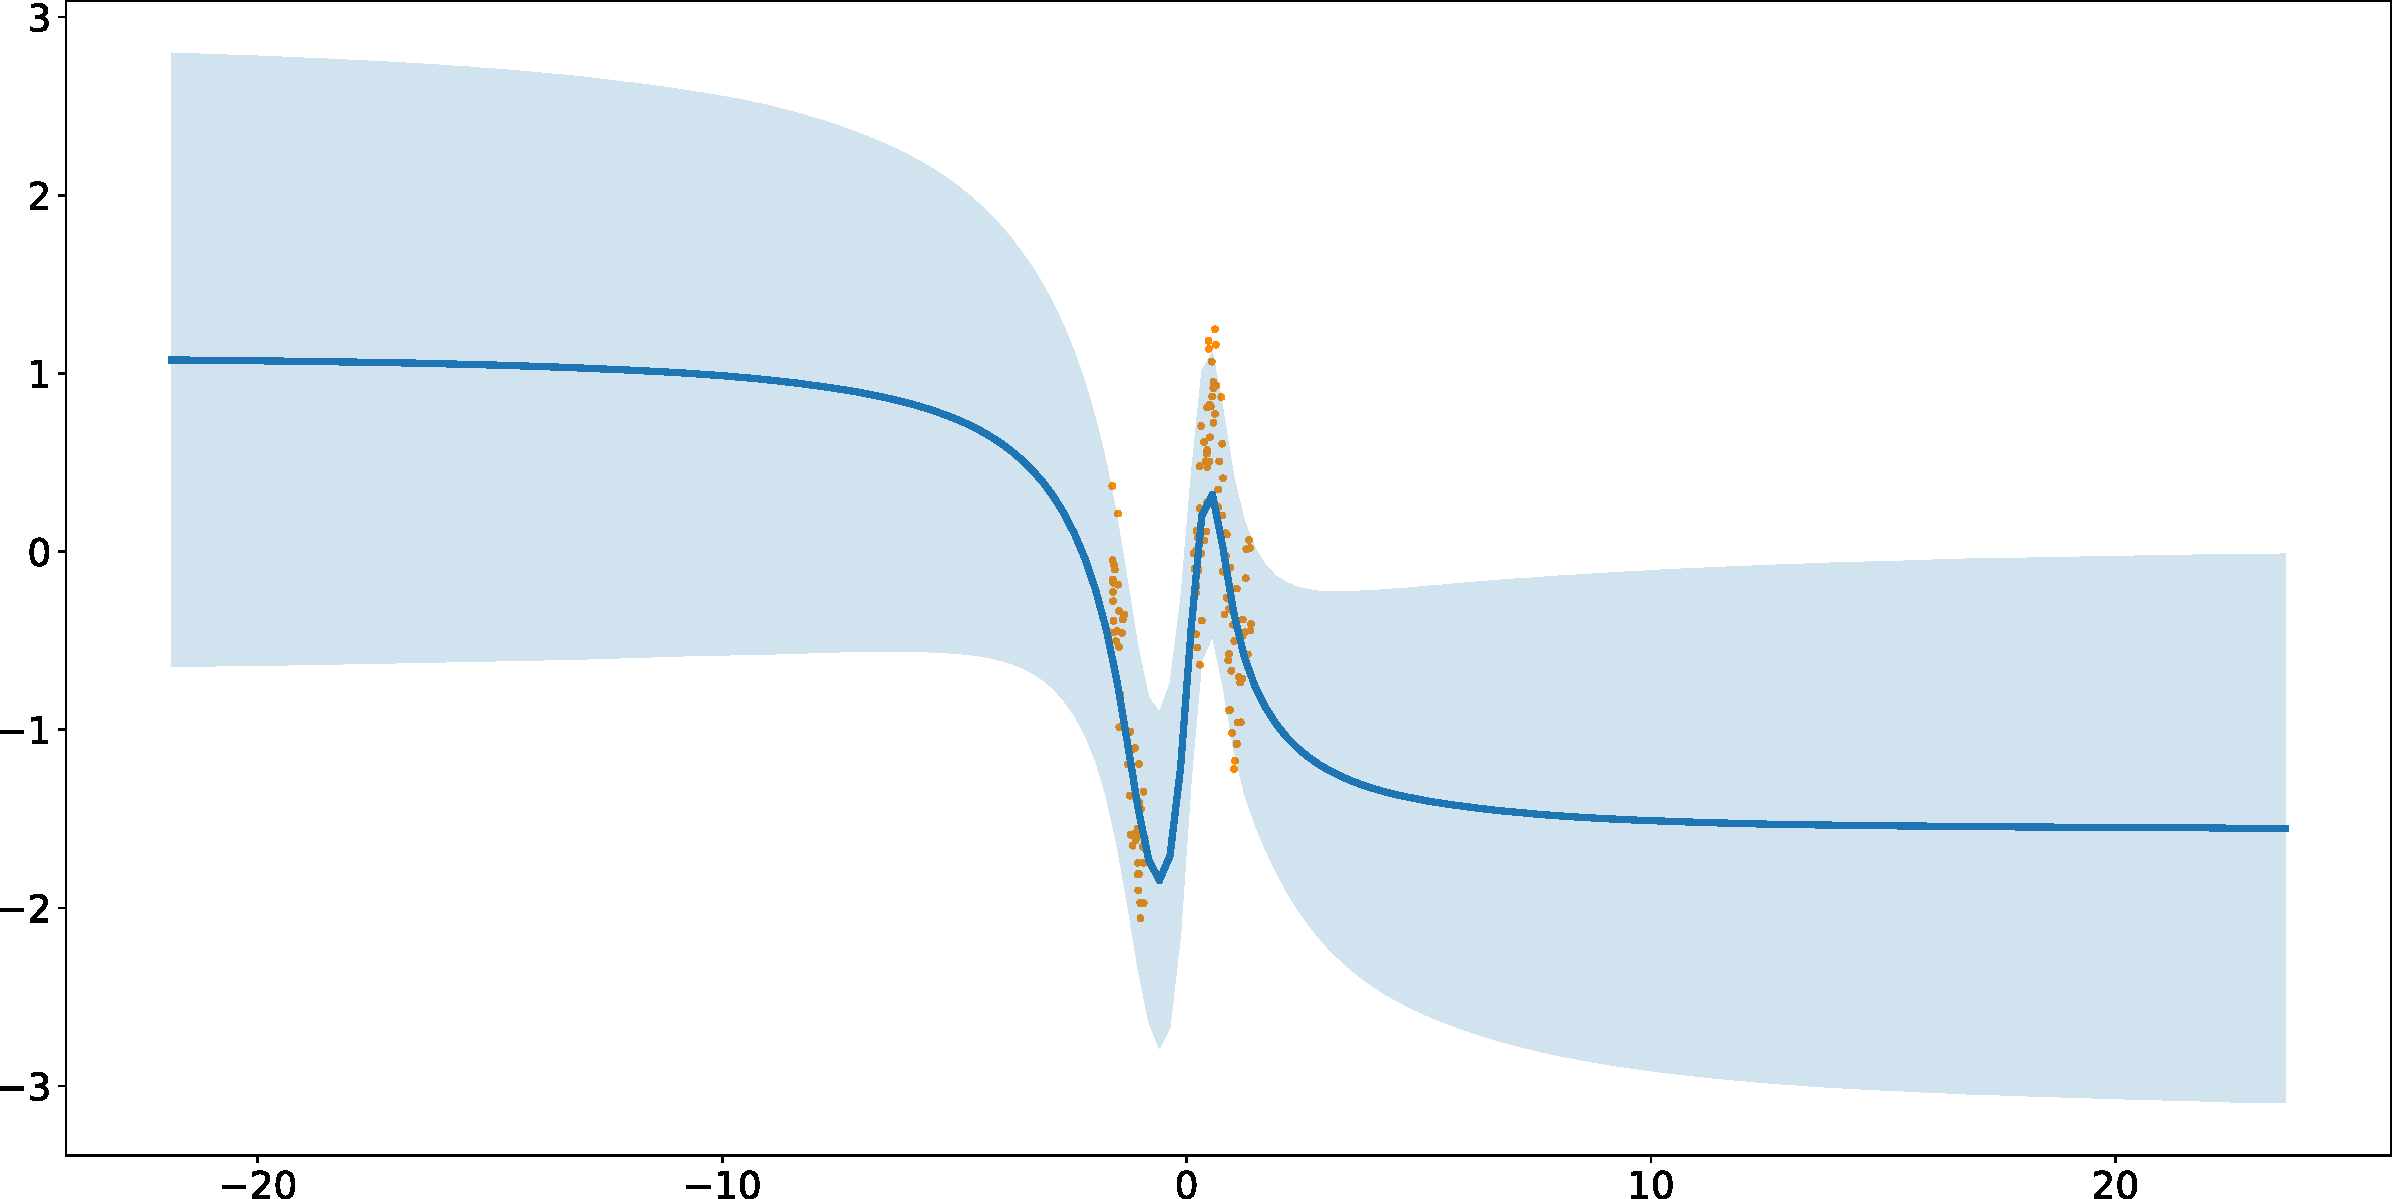
\includegraphics[width=0.49\textwidth]{imgs/Exact_GP_moments.pdf}\\  
        \end{tabular}
        \end{center}
        \begin{center}
        \begin{tabular}{ c}
         GP Taylor \\ 
         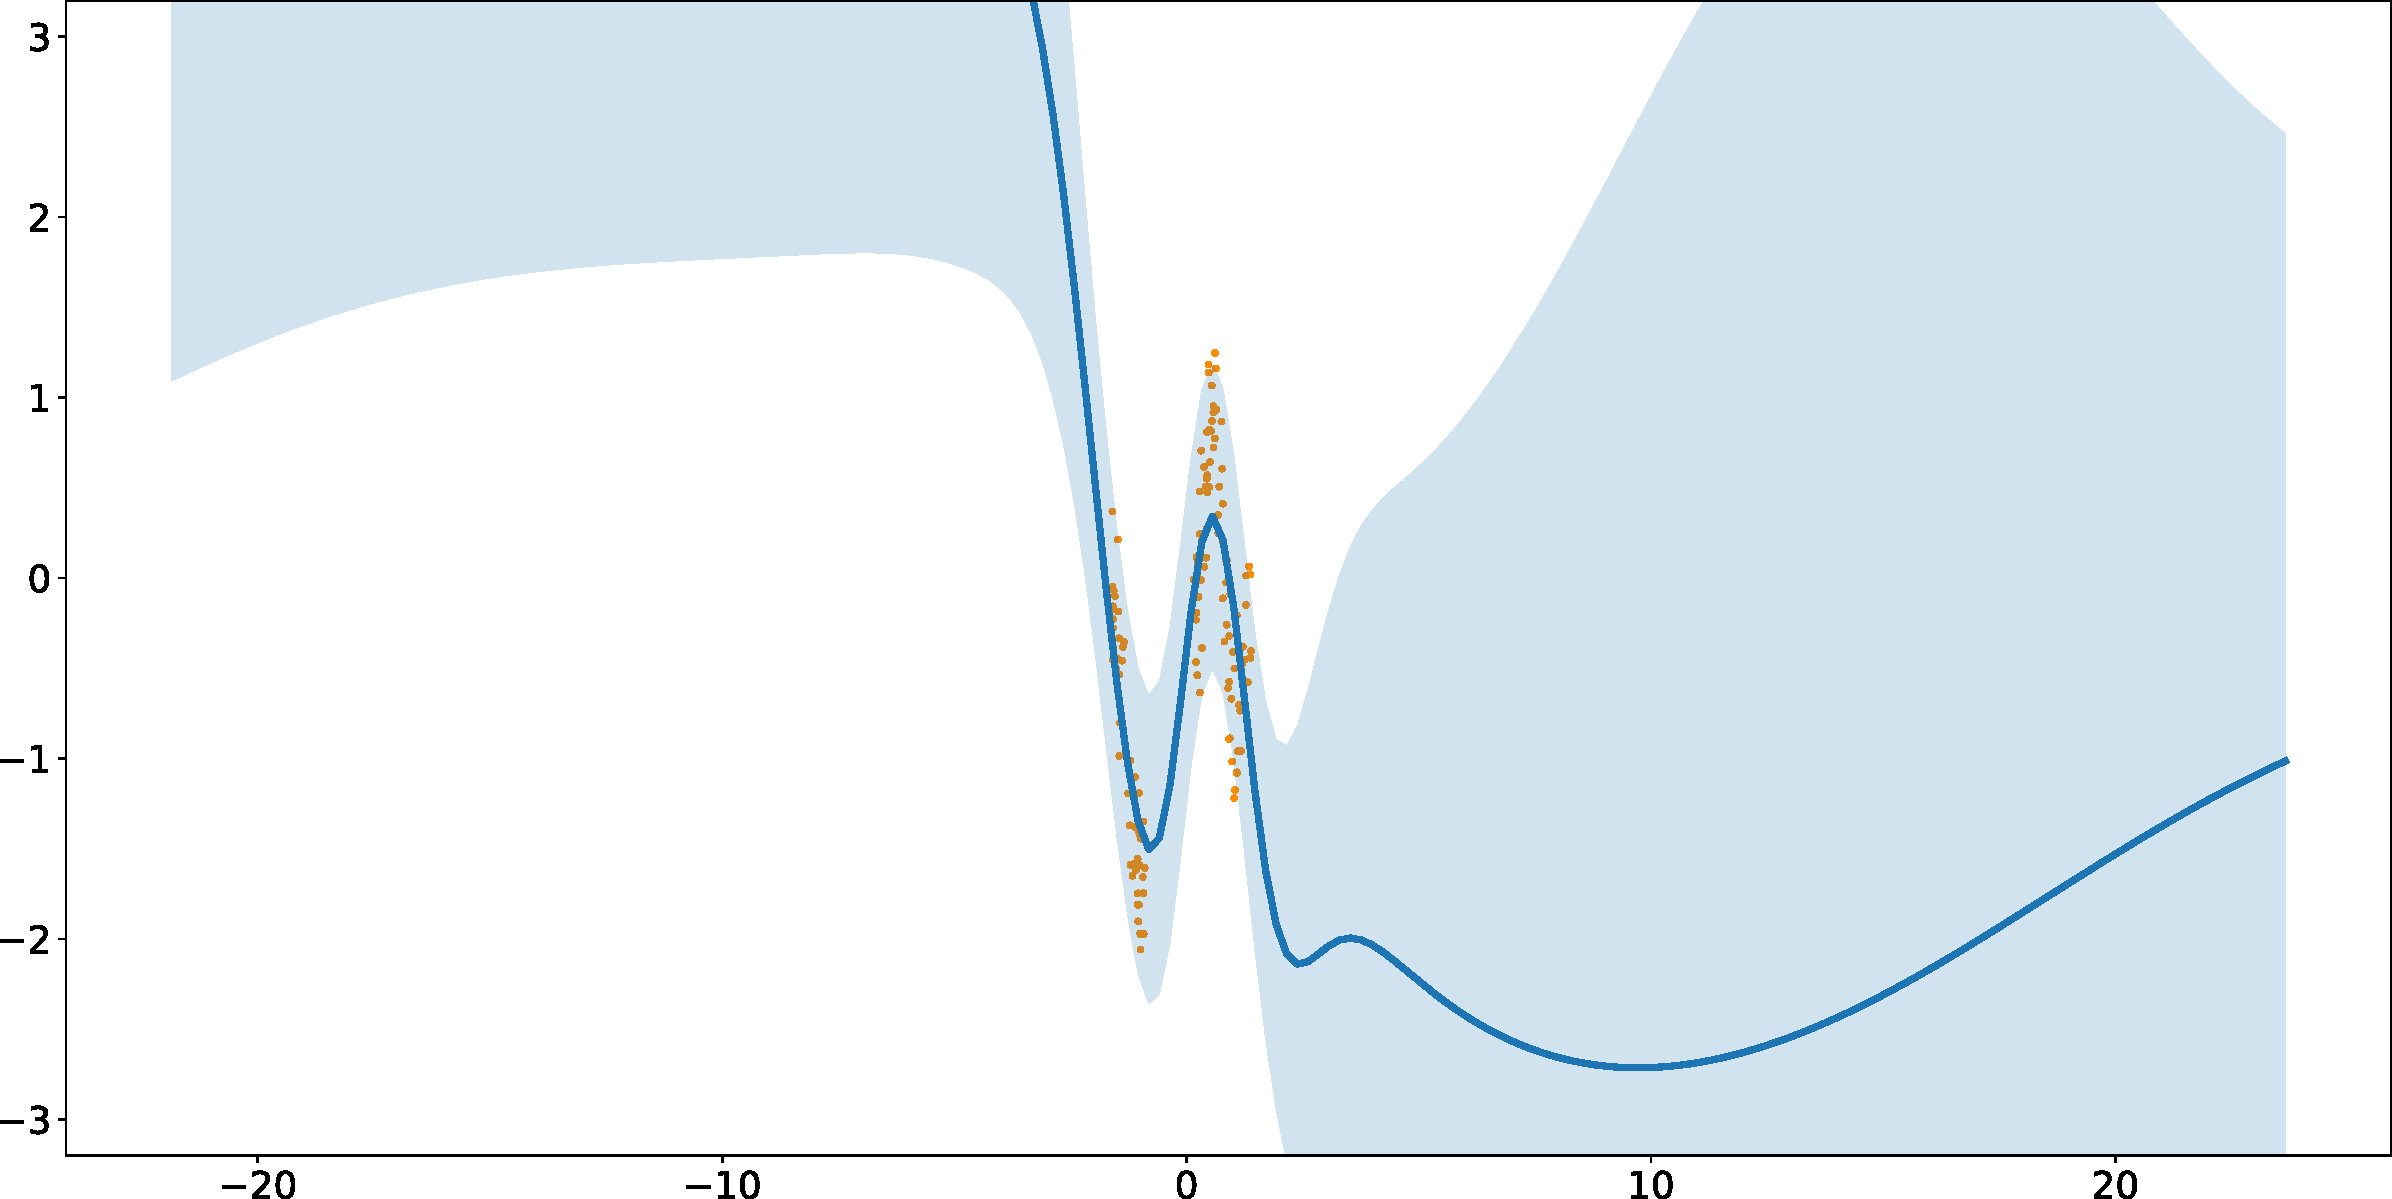
\includegraphics[width=0.49\textwidth]{imgs/Exact_GP_taylor.pdf}\\  
        \end{tabular}
        \end{center}
    \end{frame}